% Created by tikzDevice version 0.12.6 on 2026-06-17 14:28:46
% !TEX encoding = UTF-8 Unicode
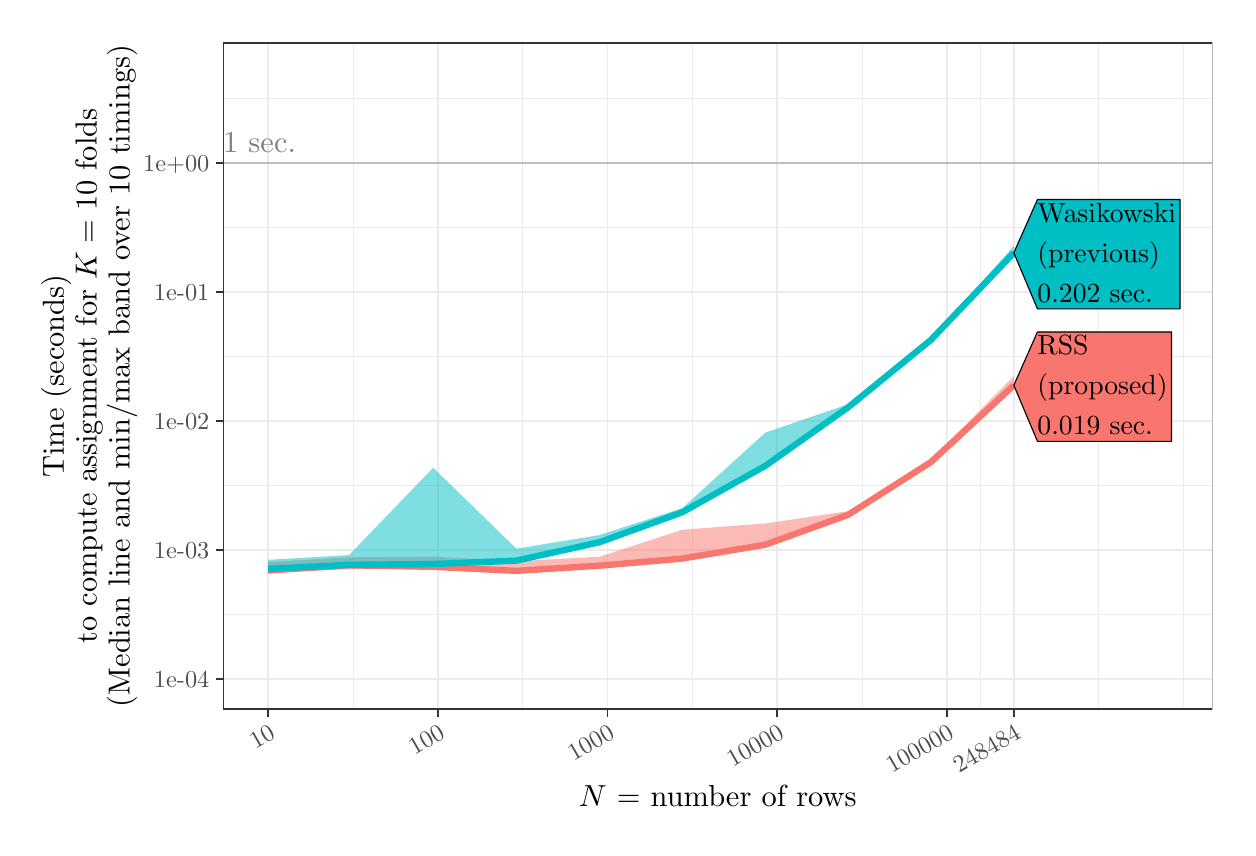
\begin{tikzpicture}[x=1pt,y=1pt]
\definecolor{fillColor}{RGB}{255,255,255}
\path[use as bounding box,fill=fillColor,fill opacity=0.00] (0,0) rectangle (433.62,289.08);
\begin{scope}
\path[clip] (  0.00,  0.00) rectangle (433.62,289.08);
\definecolor{drawColor}{RGB}{255,255,255}
\definecolor{fillColor}{RGB}{255,255,255}

\path[draw=drawColor,line width= 0.6pt,line join=round,line cap=round,fill=fillColor] (  0.00,  0.00) rectangle (433.62,289.08);
\end{scope}
\begin{scope}
\path[clip] ( 70.62, 42.84) rectangle (428.12,283.58);
\definecolor{fillColor}{RGB}{255,255,255}

\path[fill=fillColor] ( 70.62, 42.84) rectangle (428.12,283.58);
\definecolor{drawColor}{gray}{0.92}

\path[draw=drawColor,line width= 0.3pt,line join=round] ( 70.62, 77.07) --
	(428.12, 77.07);

\path[draw=drawColor,line width= 0.3pt,line join=round] ( 70.62,123.65) --
	(428.12,123.65);

\path[draw=drawColor,line width= 0.3pt,line join=round] ( 70.62,170.22) --
	(428.12,170.22);

\path[draw=drawColor,line width= 0.3pt,line join=round] ( 70.62,216.80) --
	(428.12,216.80);

\path[draw=drawColor,line width= 0.3pt,line join=round] ( 70.62,263.37) --
	(428.12,263.37);

\path[draw=drawColor,line width= 0.3pt,line join=round] (117.53, 42.84) --
	(117.53,283.58);

\path[draw=drawColor,line width= 0.3pt,line join=round] (178.84, 42.84) --
	(178.84,283.58);

\path[draw=drawColor,line width= 0.3pt,line join=round] (240.14, 42.84) --
	(240.14,283.58);

\path[draw=drawColor,line width= 0.3pt,line join=round] (301.45, 42.84) --
	(301.45,283.58);

\path[draw=drawColor,line width= 0.3pt,line join=round] (344.22, 42.84) --
	(344.22,283.58);

\path[draw=drawColor,line width= 0.3pt,line join=round] (387.00, 42.84) --
	(387.00,283.58);

\path[draw=drawColor,line width= 0.3pt,line join=round] (417.65, 42.84) --
	(417.65,283.58);

\path[draw=drawColor,line width= 0.6pt,line join=round] ( 70.62, 53.78) --
	(428.12, 53.78);

\path[draw=drawColor,line width= 0.6pt,line join=round] ( 70.62,100.36) --
	(428.12,100.36);

\path[draw=drawColor,line width= 0.6pt,line join=round] ( 70.62,146.93) --
	(428.12,146.93);

\path[draw=drawColor,line width= 0.6pt,line join=round] ( 70.62,193.51) --
	(428.12,193.51);

\path[draw=drawColor,line width= 0.6pt,line join=round] ( 70.62,240.08) --
	(428.12,240.08);

\path[draw=drawColor,line width= 0.6pt,line join=round] ( 86.87, 42.84) --
	( 86.87,283.58);

\path[draw=drawColor,line width= 0.6pt,line join=round] (148.18, 42.84) --
	(148.18,283.58);

\path[draw=drawColor,line width= 0.6pt,line join=round] (209.49, 42.84) --
	(209.49,283.58);

\path[draw=drawColor,line width= 0.6pt,line join=round] (270.80, 42.84) --
	(270.80,283.58);

\path[draw=drawColor,line width= 0.6pt,line join=round] (332.11, 42.84) --
	(332.11,283.58);

\path[draw=drawColor,line width= 0.6pt,line join=round] (356.34, 42.84) --
	(356.34,283.58);
\definecolor{drawColor}{gray}{0.50}

\node[text=drawColor,anchor=base west,inner sep=0pt, outer sep=0pt, scale=  1.10] at ( 70.62,243.87) { 1 sec.};
\definecolor{drawColor}{RGB}{190,190,190}

\path[draw=drawColor,line width= 0.6pt,line join=round] ( 70.62,240.08) -- (428.12,240.08);
\definecolor{fillColor}{RGB}{248,118,109}

\path[fill=fillColor,fill opacity=0.50] ( 86.87, 95.97) --
	(116.13, 97.70) --
	(146.53, 97.94) --
	(176.62, 96.29) --
	(206.63, 97.89) --
	(236.57,107.65) --
	(266.52,109.92) --
	(296.46,114.35) --
	(326.40,133.03) --
	(356.34,163.13) --
	(356.34,159.58) --
	(326.40,131.97) --
	(296.46,112.57) --
	(266.52,101.73) --
	(236.57, 96.42) --
	(206.63, 94.27) --
	(176.62, 92.57) --
	(146.53, 93.67) --
	(116.13, 93.39) --
	( 86.87, 92.25) --
	cycle;

\path[] ( 86.87, 95.97) --
	(116.13, 97.70) --
	(146.53, 97.94) --
	(176.62, 96.29) --
	(206.63, 97.89) --
	(236.57,107.65) --
	(266.52,109.92) --
	(296.46,114.35) --
	(326.40,133.03) --
	(356.34,163.13);

\path[] (356.34,159.58) --
	(326.40,131.97) --
	(296.46,112.57) --
	(266.52,101.73) --
	(236.57, 96.42) --
	(206.63, 94.27) --
	(176.62, 92.57) --
	(146.53, 93.67) --
	(116.13, 93.39) --
	( 86.87, 92.25);
\definecolor{fillColor}{RGB}{0,191,196}

\path[fill=fillColor,fill opacity=0.50] ( 86.87, 96.78) --
	(116.13, 98.50) --
	(146.53,130.07) --
	(176.62,100.81) --
	(206.63,105.74) --
	(236.57,115.47) --
	(266.52,142.73) --
	(296.46,153.00) --
	(326.40,176.79) --
	(356.34,210.18) --
	(356.34,207.33) --
	(326.40,175.91) --
	(296.46,151.32) --
	(266.52,130.16) --
	(236.57,113.66) --
	(206.63,102.86) --
	(176.62, 96.13) --
	(146.53, 94.36) --
	(116.13, 94.36) --
	( 86.87, 92.77) --
	cycle;

\path[] ( 86.87, 96.78) --
	(116.13, 98.50) --
	(146.53,130.07) --
	(176.62,100.81) --
	(206.63,105.74) --
	(236.57,115.47) --
	(266.52,142.73) --
	(296.46,153.00) --
	(326.40,176.79) --
	(356.34,210.18);

\path[] (356.34,207.33) --
	(326.40,175.91) --
	(296.46,151.32) --
	(266.52,130.16) --
	(236.57,113.66) --
	(206.63,102.86) --
	(176.62, 96.13) --
	(146.53, 94.36) --
	(116.13, 94.36) --
	( 86.87, 92.77);
\definecolor{drawColor}{RGB}{248,118,109}

\path[draw=drawColor,line width= 2.3pt,line join=round] ( 86.87, 92.91) --
	(116.13, 94.81) --
	(146.53, 94.25) --
	(176.62, 92.80) --
	(206.63, 94.66) --
	(236.57, 97.25) --
	(266.52,102.24) --
	(296.46,113.05) --
	(326.40,132.12) --
	(356.34,159.85);
\definecolor{drawColor}{RGB}{0,191,196}

\path[draw=drawColor,line width= 2.3pt,line join=round] ( 86.87, 93.52) --
	(116.13, 94.99) --
	(146.53, 95.27) --
	(176.62, 96.50) --
	(206.63,103.14) --
	(236.57,113.99) --
	(266.52,130.74) --
	(296.46,151.88) --
	(326.40,176.27) --
	(356.34,207.71);
\end{scope}
\begin{scope}
\path[clip] ( 70.62, 42.84) rectangle (428.12,283.58);
\definecolor{drawColor}{RGB}{0,0,0}
\definecolor{fillColor}{RGB}{248,118,109}

\path[draw=drawColor,line width= 0.4pt,line join=round,line cap=round,fill=fillColor] (356.34,159.85) --
	(364.88,179.12) --
	(413.32,179.12) --
	(413.32,139.61) --
	(364.88,139.61) --
	cycle;
\definecolor{fillColor}{RGB}{0,191,196}

\path[draw=drawColor,line width= 0.4pt,line join=round,line cap=round,fill=fillColor] (356.34,207.71) --
	(364.88,226.98) --
	(416.40,226.98) --
	(416.40,187.47) --
	(364.88,187.47) --
	cycle;

\node[text=drawColor,anchor=base west,inner sep=0pt, outer sep=0pt, scale=  1.00] at (364.88,170.81) {RSS};

\node[text=drawColor,anchor=base west,inner sep=0pt, outer sep=0pt, scale=  1.00] at (364.88,156.41) {(proposed)};

\node[text=drawColor,anchor=base west,inner sep=0pt, outer sep=0pt, scale=  1.00] at (364.88,142.01) {0.019 sec.};

\node[text=drawColor,anchor=base west,inner sep=0pt, outer sep=0pt, scale=  1.00] at (364.88,218.67) {Wasikowski};

\node[text=drawColor,anchor=base west,inner sep=0pt, outer sep=0pt, scale=  1.00] at (364.88,204.27) {(previous)};

\node[text=drawColor,anchor=base west,inner sep=0pt, outer sep=0pt, scale=  1.00] at (364.88,189.87) {0.202 sec.};
\definecolor{drawColor}{gray}{0.20}

\path[draw=drawColor,line width= 0.6pt,line join=round,line cap=round] ( 70.62, 42.84) rectangle (428.12,283.58);
\end{scope}
\begin{scope}
\path[clip] (  0.00,  0.00) rectangle (433.62,289.08);
\definecolor{drawColor}{gray}{0.30}

\node[text=drawColor,anchor=base east,inner sep=0pt, outer sep=0pt, scale=  0.88] at ( 65.67, 50.75) {1e-04};

\node[text=drawColor,anchor=base east,inner sep=0pt, outer sep=0pt, scale=  0.88] at ( 65.67, 97.33) {1e-03};

\node[text=drawColor,anchor=base east,inner sep=0pt, outer sep=0pt, scale=  0.88] at ( 65.67,143.90) {1e-02};

\node[text=drawColor,anchor=base east,inner sep=0pt, outer sep=0pt, scale=  0.88] at ( 65.67,190.48) {1e-01};

\node[text=drawColor,anchor=base east,inner sep=0pt, outer sep=0pt, scale=  0.88] at ( 65.67,237.05) {1e+00};
\end{scope}
\begin{scope}
\path[clip] (  0.00,  0.00) rectangle (433.62,289.08);
\definecolor{drawColor}{gray}{0.20}

\path[draw=drawColor,line width= 0.6pt,line join=round] ( 67.87, 53.78) --
	( 70.62, 53.78);

\path[draw=drawColor,line width= 0.6pt,line join=round] ( 67.87,100.36) --
	( 70.62,100.36);

\path[draw=drawColor,line width= 0.6pt,line join=round] ( 67.87,146.93) --
	( 70.62,146.93);

\path[draw=drawColor,line width= 0.6pt,line join=round] ( 67.87,193.51) --
	( 70.62,193.51);

\path[draw=drawColor,line width= 0.6pt,line join=round] ( 67.87,240.08) --
	( 70.62,240.08);
\end{scope}
\begin{scope}
\path[clip] (  0.00,  0.00) rectangle (433.62,289.08);
\definecolor{drawColor}{gray}{0.20}

\path[draw=drawColor,line width= 0.6pt,line join=round] ( 86.87, 40.09) --
	( 86.87, 42.84);

\path[draw=drawColor,line width= 0.6pt,line join=round] (148.18, 40.09) --
	(148.18, 42.84);

\path[draw=drawColor,line width= 0.6pt,line join=round] (209.49, 40.09) --
	(209.49, 42.84);

\path[draw=drawColor,line width= 0.6pt,line join=round] (270.80, 40.09) --
	(270.80, 42.84);

\path[draw=drawColor,line width= 0.6pt,line join=round] (332.11, 40.09) --
	(332.11, 42.84);

\path[draw=drawColor,line width= 0.6pt,line join=round] (356.34, 40.09) --
	(356.34, 42.84);
\end{scope}
\begin{scope}
\path[clip] (  0.00,  0.00) rectangle (433.62,289.08);
\definecolor{drawColor}{gray}{0.30}

\node[text=drawColor,rotate= 30.00,anchor=base east,inner sep=0pt, outer sep=0pt, scale=  0.88] at ( 89.90, 32.64) {10};

\node[text=drawColor,rotate= 30.00,anchor=base east,inner sep=0pt, outer sep=0pt, scale=  0.88] at (151.21, 32.64) {100};

\node[text=drawColor,rotate= 30.00,anchor=base east,inner sep=0pt, outer sep=0pt, scale=  0.88] at (212.52, 32.64) {1000};

\node[text=drawColor,rotate= 30.00,anchor=base east,inner sep=0pt, outer sep=0pt, scale=  0.88] at (273.83, 32.64) {10000};

\node[text=drawColor,rotate= 30.00,anchor=base east,inner sep=0pt, outer sep=0pt, scale=  0.88] at (335.14, 32.64) {100000};

\node[text=drawColor,rotate= 30.00,anchor=base east,inner sep=0pt, outer sep=0pt, scale=  0.88] at (359.37, 32.64) {248484};
\end{scope}
\begin{scope}
\path[clip] (  0.00,  0.00) rectangle (433.62,289.08);
\definecolor{drawColor}{RGB}{0,0,0}

\node[text=drawColor,anchor=base,inner sep=0pt, outer sep=0pt, scale=  1.10] at (249.37,  7.64) {$N$ = number of rows};
\end{scope}
\begin{scope}
\path[clip] (  0.00,  0.00) rectangle (433.62,289.08);
\definecolor{drawColor}{RGB}{0,0,0}

\node[text=drawColor,rotate= 90.00,anchor=base,inner sep=0pt, outer sep=0pt, scale=  1.10] at ( 13.08,163.21) {Time (seconds)};

\node[text=drawColor,rotate= 90.00,anchor=base,inner sep=0pt, outer sep=0pt, scale=  1.10] at ( 24.96,163.21) {to compute assignment for $K=10$ folds};

\node[text=drawColor,rotate= 90.00,anchor=base,inner sep=0pt, outer sep=0pt, scale=  1.10] at ( 36.84,163.21) {(Median line and min/max band over 10 timings)};
\end{scope}
\end{tikzpicture}
